\newpage
\begin{song}{title={Press gang (Branka)}, music={Cztery refy}}
\begin{multicols}{2}
    \begin{verse}
        W dół od rzeki, poprzez London Street\\
		Psów królewskich oddział zwarty szedł\\
		Ojczyźnie trzeba dziś świeżej krwi\\
		Marynarzy floty wojennej\\
    \end{verse}
    \begin{verse}
       A że byłem wtedy silny chłop\\
       W tłumie złowił mnie sierżanta wzrok \\
       W kajdanach z bramy wywlekli mnie \\
       Marynarza floty wojennej \\
    \end{verse}
    \begin{verse}
    Jak o prawa upominać się \\
    Na gretingu nauczyli mnie \\
    Niejeden krwią wtedy spłynął grzbiet \\
    Marynarza floty wojennej \\
    \end{verse}
    \begin{verse}
	Nikt nie zliczy ile krwi i łez \\
	Wsiąkło w pokład, gdy się zaczął rejs \\
	Dla chwały twej, słodki kraju mój \\
	Marynarzy floty wojennej \\
    \end{verse}
    \begin{verse}
	Hen, za rufą miły został dom \\
	Jesteś tylko parą silnych rąk \\
	Dowódca tu twoim bogiem jest \\
	Marynarzu floty wojennej \\
    \end{verse}
    \begin{verse}
    Gdy łapaczy szyk formuje się \\
	W pierwszym rzędzie możesz ujrzeć mnie \\
	Kto stanie na mojej drodze dziś \\ 
	\textbf{Łup} stanowi floty wojennej \\
    \end{verse}
\end{multicols}
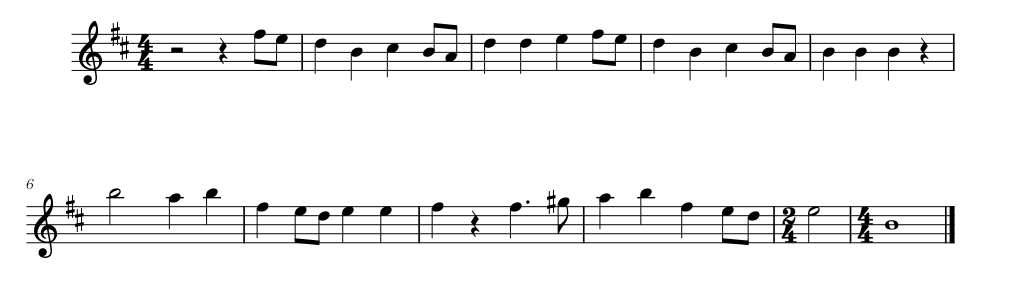
\includegraphics[width=\textwidth]{sheet_music/cztery_refy-press_gang.png}  
\end{song}
\newpage
